\documentclass[12pt, aspectratio=141]{beamer}

\definecolor{jrouge}{HTML}{CB3C33}
\definecolor{jvert}{HTML}{389826}
\definecolor{jbleu}{HTML}{4063D8}
\definecolor{jviolet}{HTML}{9558B2}
\definecolor{lightred}{HTML}{fcf3f3}
\definecolor{lightgreen}{HTML}{e1f6db}
\definecolor{lightpurple}{HTML}{f4eef7}
\definecolor{lightgrey}{gray}{0.95}

\mode<presentation>
{
	\usetheme{default}
	\usecolortheme{rose}
	%	\useoutertheme{smoothbars}
	\useinnertheme{circles}
	
	\definecolor{beamer@blendedblue}{HTML}{4063D8}
	%\definecolor{titlemustard}{rgb}{0.6,0.6,0.0}
	%\setbeamercolor{title}{bg=titlemustard}
	\setbeamercolor{normal text}{fg=black}
	\setbeamercolor{alerted text}{fg=jrouge}
	\setbeamerfont{title}{shape=\bfseries}
	\setbeamercolor{example text}{fg=jvert}
	
	%\setbeamercolor{structure}{fg=beamer@blendedblue}
	\setbeamertemplate{navigation symbols}{}
	\setbeamertemplate{footline}{\color{black!50}\hfill\scriptsize\insertpagenumber\hspace{2em}\vspace{2em}}
}

\usepackage{natbib}
%\renewcommand{\citenumfont}[1]{{\tiny#1}}
\renewcommand{\citenumfont}[1]{}
\bibpunct{}{};s;;

\usepackage[french]{babel}
\usepackage[mathletters]{ucs}
\usepackage[utf8x]{inputenc}
\usepackage[T1]{fontenc}
% Or whatever. Note that the encoding and the font should match. If T1
% does not look nice, try deleting the line with the fontenc.
% Alternative for XeLaTeX:
%\usefonttheme{professionalfonts}
%\usepackage{fontspec}
%\setmonofont{JuliaMono}
%\setdefaultlanguage{french}
%\usepackage{unicode-math}

\usepackage{subcaption}

\usepackage{array}
\usepackage{multirow}
\usepackage{setspace}
\usepackage{soul}
\usepackage{amssymb}
\usepackage{mathrsfs}
\usepackage{bbm}
\usepackage{svg}

\usepackage{tikz}
\usetikzlibrary{scopes, backgrounds, arrows, automata, positioning, patterns, calc, decorations.pathmorphing, decorations.pathreplacing, arrows.meta}

\usepackage{hyperref}
\usepackage{ragged2e}
\usepackage{graphicx}
\usepackage{amsmath}
\usepackage{aeguill}

\usepackage{algorithm}
\usepackage{algpseudocode}
\usepackage{stmaryrd}
\usepackage{moresize}

\newcommand{\llbra}{\left\llbracket}
\newcommand{\rrbra}{\right\rrbracket}
\renewcommand{\brack}[1]{\ensuremath{\llbra#1\rrbra}}
\newcommand{\der}[2]{#1^{\ensuremath{\left(#2\right)}}}
\newcommand{\paren}[1]{\ensuremath{\left(#1\right)}}
\newcommand{\abs}[1]{\ensuremath{\left|#1\right|}}
\newcommand{\interval}[1]{\ensuremath{\left[#1\right]}}
\newcommand{\set}[2]{\ensuremath{\left\{#1\,\middle|\,#2\right\}}}
\newcommand{\cont}[1]{\mathcal{C}^{#1}}
\newcommand{\tends}[2]{\underset{#1\to #2}{\longrightarrow}}
\newcommand{\seq}[3]{\ensuremath{\left(#1_{#2}\right)_{#2\in#3}}}
\newcommand{\matr}[2]{\mathcal{M}_{#1}\paren{#2}}
\newcommand{\matrRect}[3]{\mathcal{M}_{#1,#2}\paren{#3}}
\newcommand{\Id}{\text{Id}}
\newenvironment{disj}[1]{\left\{\begin{array}{#1}} {\end{array}\right.}

\usepackage{siunitx}


\newenvironment{changemargin}[2]{%
	\begin{list}{}{%
			%\setlength{\topsep}{0pt}%
			\setlength{\leftmargin}{#1}%
			\setlength{\rightmargin}{#2}%
			\setlength{\listparindent}{\parindent}%
			\setlength{\itemindent}{\parindent}%
			\setlength{\parsep}{\parskip}%
		}%
		\item[]}{\end{list}}

\defbeamertemplate{section page}{mruffel}[1][]{%
	\begin{centering}
		{\usebeamerfont{section name}\usebeamercolor[fg]{section name}#1
			\vskip1em\par
			
			\begin{beamercolorbox}[sep=12pt,center,rounded=true,shadow=true]{part title}
				\usebeamerfont{section title}\insertsection\par
		\end{beamercolorbox}}
	\end{centering}
}



% If you have a file called "university-logo-filename.xxx", where xxx
% is a graphic format that can be processed by latex or pdflatex,
% resp., then you can add a logo as follows:

\pgfdeclareimage[height=0.5cm]{Mines}{../figures/Mines.pdf}
\logo{\begin{tikzpicture}[overlay,remember picture]
		\node[left=0.2cm] at (current page.31){
			\pgfuseimage{Mines}
		};
\end{tikzpicture}}



% Delete this, if you do not want the table of contents to pop up at
% the beginning of each subsection:
%\AtBeginSubsection[]
%{
	%  \begin{frame}<beamer>
		%    \tableofcontents[currentsection,currentsubsection]
		%  \end{frame}
	%}

\AtBeginSection[]
{
	\begin{frame}
		\sectionpage
	\end{frame}
}

% If you wish to uncover everything in a step-wise fashion, uncomment
% the following command: 

%\beamerdefaultoverlayspecification{<+->}

\usepackage{minted}
\usemintedstyle{paraiso-light}
\setminted[julia]{mathescape,linenos,obeytabs,tabsize=4,numbersep=3pt,fontsize=\small,framesep=2mm,autogobble,bgcolor=lightred,escapeinside=££}
\setminted[bash]{mathescape,obeytabs,tabsize=4,numbersep=3pt,fontsize=\small,framesep=2mm,autogobble,bgcolor=lightgrey,escapeinside=££}

\usepackage{lmodern}
%\newcommand{\jl}[1]{\colorbox{lightred}{\small\ttfamily #1}}
\newmintinline[jl]{julia}{}
\newmintinline[jlscript]{julia}{fontsize=\scriptsize}
\newmint[JL]{julia}{}
\newmint[JLa]{julia}{linenos=false}
\newminted{julia}{}
\newenvironment{julia}{\vspace{-0.6em}\VerbatimEnvironment\begin{juliacode}}{\end{juliacode}}
\newminted[jlrepl]{julia}{linenos=false}
\newenvironment{repl}{\vspace{-0.6em}\VerbatimEnvironment\begin{jlrepl}}{\end{jlrepl}}
\newcommand{\q}{\textquotesingle}
\newcommand{\qq}{\textquotedbl}
\newcommand{\jlREPL}{\textcolor{jvert}{\bfseries julia>}}

\DeclareTextFontCommand{\emph}{\color{jrouge}\bfseries}

\newenvironment<>{definition}[1]{%
	\setbeamercolor{block title}{bg=lightgreen}%
	\begin{block}{Définition}{#1}}{\end{block}}

\newenvironment<>{convention}[1]{%
	\setbeamercolor{block title}{bg=lightpurple}%
	\begin{block}{Convention}{#1}}{\end{block}}

\usepackage{xspace}
\newcommand{\expr}{\ensuremath{\left\langle\textit{expr}\right\rangle}\xspace}
\newcommand{\expra}[1]{\ensuremath{\left\langle\textit{expr}_{#1}\right\rangle}\xspace}
\newcommand{\bexpr}{\ensuremath{\left\langle\textit{bexpr}\right\rangle}\xspace}
\newcommand{\bexpra}[1]{\ensuremath{\left\langle\textit{bexpr}_{#1}\right\rangle}\xspace}
\newcommand{\type}{\ensuremath{\left\langle\textit{type}\right\rangle}\xspace}
\newcommand{\typea}[1]{\ensuremath{\left\langle\textit{type}_{#1}\right\rangle}\xspace}


\title{Apprentissage de la programmation en Julia}

\subtitle{Calepins électroniques, unités physiques, figures}

\author{Lionel~Zoubritzky\inst{}}

\institute{Mines Paris -- PSL}

\date{12/2024}

\begin{document}
\setbeamertemplate{section page}[mruffel]

\begin{frame}
	\titlepage
\end{frame}


\section{Calepins électroniques}


\begin{frame}{Calepin électronique}
	\begin{definition}
		Un \emph{calepin électronique} (\textit{notebook}) est un fichier qui contient un mélange de code, de texte, et parfois de contenus multimédias (images, sons, vidéos).
	\end{definition}
	\vfill

	Mettre son code dans un calepin électronique permet de disposer son code à côté de ses résultats, et de toute sorte de documentation ou d'éléments utiles à la compréhension.
	\vfill

	Il s'agit d'une bonne pratique pour du code au stade de prototype par exemple. Pour du code de production, on préférera créer un logiciel ou une bibliothèque ({\footnotesize\url{https://pkgdocs.julialang.org/v1/creating-packages/}}).
\end{frame}

\begin{frame}{Cellules}
	Un calepin est divisée en \emph{cellules}. Il en existe généralement deux sortes :
	\begin{itemize}
		\item Une cellule de code contient du code.
		\item Une cellule de \emph{Markdown} contient du texte, au format Markdown :
		\begin{itemize}
			\item \texttt{\LARGE \# Premier niveau de titre},\\ \texttt{\Large \#\# Deuxième}, \texttt{\large \#\#\# Troisième}, \texttt{\#\#\#\# Quatrième}, \ldots
			\vspace{0.4em}
			
			\item Le texte normal est écrit tel quel.
			\vspace{0.4em}

			\item \texttt{*\textit{Emphase}*}, \texttt{**\mbox{\textbf{Gras}\hspace{0.03mm}\llap{\textbf{Gras}}\hspace{0.03mm}\llap{\textbf{Gras}}\hspace{0.03mm}\llap{\textbf{Gras}}}**}, \texttt{\_\textit{Italique}\_} \texttt{\textasciitilde\st{Barr\'e}\textasciitilde}
			\vspace{0.4em}

			\item \texttt{- Une liste\\ - à puces}
			\vspace{0.4em}

			\item \texttt{1. Une\\ 2. liste\\ 3. numérotée}
			\vspace{0.4em}
			
			\item \LaTeX: \texttt{\$\$\textbackslash frac\{\textbackslash pi\textasciicircum2\}6 = \textbackslash sum\_\{i=1\}\textasciicircum\textbackslash infty\textbackslash frac1\{i\textasciicircum2\}\$\$}
			\vspace{0.4em}

			\item \texttt{\textasciigrave f(x) = "mon code"\textasciigrave}
			\vspace{0.4em}

			\item \texttt{[nom du lien](https://url/d/un/site/web)}
			\vspace{0.4em}

			\item et d'autres : voir \scriptsize\url{https://featured.plutojl.org/basic/markdown}
		\end{itemize}
	\end{itemize}
\end{frame}

\begin{frame}{Jupyter notebook}
	Les calepins électroniques les plus communs sont ceux basés sur l'architecture Jupyter.

	{\footnotesize Note : ``Ju'' $\Rightarrow$ Julia ; ``pyt'' $\Rightarrow$ Python ; ``er'' $\Rightarrow$ R}
	\vfill

	Jupyter est facile à prendre en main, et très utilisé dans la communauté Python (en particulier pour les sciences des données).\\

	Pour inclure du code Julia dans un Jupyter notebook, il faut installer l'environnement de développement Jupyter, inclus dans Anaconda par exemple, ainsi que la bibliothèque IJulia.jl en Julia.
	\vfill
\end{frame}

\begin{frame}{Pluto}
	Julia dispose de son propre système de calepins électoniques grâce à la bibliothèque Pluto.jl.
	\vfill
	
	\begin{block}{Environnement réactif}
		La différence majeure entre les calepins de Jupyter et de Pluto est que Pluto propose un environnement \emph{réactif}. Cela signifie que toute modification dans une cellule est immédiatement répercutée sur toutes les autres cellules.
	\end{block}
	\vfill

	Ce comportement réactif rend Pluto particulièrement utile pour analyser des situations physiques qui dépendent de paramètres : il suffit de faire varier les paramètres pour voir l'effet directement.
	\vfill
	
	Cela permet aussi d'éviter des erreurs dues à un ordre spécifique d'exécution des cellules. Il est en effet impossible de spécifier l'ordre d'exécution des cellules en Pluto.
\end{frame}

\begin{frame}{Exécution et stockage d'un calepin électronique}
	Pour exécuter une cellule, on utilise le raccourci Maj+Entrée.\\
	Pour exécuter et créer une nouvelle cellule, on utilise Ctrl+Entrée.\\
	Le résultat de l'exécution est affiché \textbf{au dessus} de la cellule en Pluto. En Jupyter, il est affiché en dessous.\\
	
	Les Pluto notebooks ne stockent \textbf{pas} les résultats de l'exécution des cellules. Ils doivent donc être exécutés à chaque fois qu'ils sont ouverts.
	
	Cela les force à être parfaitement reproductibles. Cela diminue par ailleurs leur taille, ce qui permet de les stocker sur GitHub par exemple.\\
	
	Inversement, les Jupyter notebooks stockent le résultat de l'exécution.\\
	
	Dans Pluto, appuyer sur F1 permet d'afficher l'aide (dans Jupyter : H)
\end{frame}

\begin{frame}[fragile]{Markdown dans Pluto}
	En Pluto, il n'y a pas de cellule Markdown : toutes les cellules sont du code Julia. Pour afficher du Markdown, on l'encapsule dans une chaîne de caractère précédée par \jl{md} (raccourci : Ctrl+M) :
	
	\begin{minted}{julia}
		md"""
		This is my Markdown comment. I can do interpolation: `x = $x`
		"""
	\end{minted}
	\vfill
	
	Après avoir exécuté la cellule contenant Markdown, il vaut mieux cacher son code pour ne plus voir que son affichage : il faut pour taper Ctrl+Maj+[ ou cliquer sur \includegraphics[height=1em]{../figures/eye-pluto.pdf}. Pour faire l'opération inverse, Ctrl+Maj+] ou re-cliquer sur \includegraphics[height=1em]{../figures/eye-pluto.pdf}.
	\vfill
	
	Pour plus d'aide, consulter : \footnotesize\url{https://featured.plutojl.org/basic/markdown}
\end{frame}

\begin{frame}{Interactivité dans Pluto}
	Un grand avantage de Pluto est la possibilité de changer à la volée des valeurs de paramètres. Pour cela, on utilise la bibliothèque PlutoUI.jl, qui fournit la macro \jl{bind}.
	\begin{itemize}
		\item \jl{@bind var Slider(rnge; [default=])} permet de choisir la valeur pour la variable \jl{var} parmi un \textbf{intervalle} \jl{rnge}. Une valeur par défaut peut être passée optionellement.
		
		\jl{Slider} peut être remplacé par \jl{NumberField} pour afficher la valeur de \jl{var} à la place de celle de l'intervalle.
		\item \jl{@bind var CheckBox([; default=]} permet de choisir une valeur \textbf{booléenne} pour la variable \jl{var} grâce à une case à cocher.
		\item \jl{@bind var Select(list)} permet de choisir une valeur pour la variable \jl{var} parmi une liste d'options.
	\end{itemize}
	\vfill

	Pour plus d'options : \footnotesize\url{https://featured.plutojl.org/basic/plutoui.jl}
\end{frame}


\section{Unités physiques}


\begin{frame}{Unitful}
	La bibliothèque Unitful.jl permet d'exprimer des grandeurs physiques avec leurs unités en Julia.
	\vfill
	
	Pour cela, il suffit de multiplier la valeur par son unité, écrite dans une chaîne de caractère précédée par un \jl{u}. Par exemple :
	\begin{itemize}
		\item \jl{u"m^2/kg"} est l'unité \unit{m^2/kg}.
		\item \jl{3.5u"cm^(1/2)"} représente \qty{3,5}{cm^{1/2}}.
		\item Un tableau peut aussi être multiplié par une unité pour donner l'unité à chaque élément du tableau : \jl{[1.0, 2.5]u"rad*s^-1"}.
	\end{itemize}
	\vfill

	Pour vérifier si un nombre a une unité, on vérifie son type : \jl{2.4u"kg"} est une instance de \jl{Quantity} (qui vient de Unitful.jl) et de \jl{Number}, mais pas de \jl{Real}.
\end{frame}

\begin{frame}[fragile]{Homogénéité et conversion}
	Les opérations inhomogènes lancent des erreurs :
	\begin{repl}
		£\jlREPL£ 3u"s" + 2u"kg"
		ERROR: DimensionError: 3 s and 2 kg are not dimensionally
		compatible.
	\end{repl}
	\vfill

	Les conversions d'unité ont lieu automatiquement lorsque nécessaire :
	\begin{repl}
		£\jlREPL£ 3u"s" + 2u"ms"
		1501//500 s

		£\jlREPL£ 3.5u"cm^3" + 2u"L"
		0.0020035 m^3
	\end{repl}
	\vfill
	
	Il est aussi possible de demander une conversion explicitement :
	\begin{repl}
		£\jlREPL£ uconvert(u"J/hr", 12.0u"W")
		43200.0 J hr^-1
	\end{repl}
\end{frame}

\begin{frame}[fragile]{Suppression d'unité}
	Pour manipuler le nombre sans l'unité, on utiliser \jl{ustrip} avec l'unité attendue en premier argument:
	\begin{repl}
		£\jlREPL£ ustrip(u"°C", 27u"°C")
		27
		
		£\jlREPL£ ustrip(u"J/cm^2", 13.5e-7u"bar*km")
		0.0135
	\end{repl}
	
	\jl{NoUnits} désigne l'unité des grandeurs\ldots sans unité !
	\begin{repl}
		£\jlREPL£ x = 5u"°/rad"
		5 ° rad^-1
		
		£\jlREPL£ ustrip(NoUnits, x)
		0.08726646259971647

		£\jlREPL£ NoUnits(x) # more explicit alternative
		0.08726646259971647
	\end{repl}
\end{frame}


\section{Figures}


\begin{frame}{Principe}
	La production de \emph{figures} est essentielle dans la plupart des métiers de l'ingénieur et de la recherche.
	\vfill

	\textbf{Une figure doit exprimer une idée clairement.}
	\vfill

	Les figures contiennent généralement des données quantifiées. Si ce n'est pas le cas, on parle de schéma (en général, mieux vaut utiliser un outil de dessin non programmatique comme Inkscape pour ceux-ci).
\end{frame}

\begin{frame}{Bibliothèques de dessin de figures}
	Il existe plusieurs bibliothèques pour le dessin scientifique en Julia :
	\begin{itemize}
		\item \texttt{Makie.jl}, le sujet de ce cours ;
		\item \texttt{Plots.jl}, proche de \texttt{matplotlib} en Python ;
		\item \texttt{AlgebraOfGraphics.jl} et \texttt{Gadfly.jl}, proches de \texttt{ggplot2} en R ;
		\item \texttt{UnicodePlots.jl} pour afficher dans le REPL ;
		\item \texttt{Gaston.jl}, \texttt{PGFPlotsX.jl}, \texttt{Vega.jl}, et d'autres\ldots
	\end{itemize}
	\vfill

	On se concentre sur \texttt{Makie.jl}, le plus complet et probablement le plus utilisé dans un futur proche.
\end{frame}

\begin{frame}{Bibliothèques de dessin de figures}
	\centering
	\includegraphics[width=\linewidth]{../figures/plotting_libraries.png}
\end{frame}

\begin{frame}{Backend}
	\texttt{Makie.jl} (tout comme \texttt{Plots.jl}) est une bibliothèque qui spécifie une \emph{interface} pour le dessin scientifique. Cette interface est implémentée par des \emph{backends} : on n'appelle donc pas la bibliothèque par la commande \jl{using Makie}, mais à la place on appelle le backend directement. Le choix est :
	\begin{itemize}
		\item \texttt{CairoMakie.jl} : la meilleure qualité ;
		\item \texttt{GLMakie.jl} et \texttt{WGLMakie.jl} : interactifs ;
		\item \texttt{RPRMakie.jl} : ray-tracing, pour applications spécifiques ;
	\end{itemize}
	\vfill

	On suppose dans le reste du cours que la commande suivante a été exécutée (il faut donc l'inclure dans le fichier \texttt{***.jl}) : \vspace{-0.6em}
	\JL{using GLMakie}
	(On peut aussi utiliser \jl{using GLMakie} ou \jl{using WGLMakie} à la place.)
\end{frame}

\begin{frame}{Données linéaires simples}
	Pour les données qui s'expriment comme un ensemble de points $(x_i, y_i)_{i\in I}$, on affiche ces points avec l'une des trois fonctions :
	\begin{itemize}
		\item \jl{scatter} : chaque point est affiché individuellement ;
		\item \jl{lines} : les points sont liés entre eux ;
		\item \jl{scatterlines} : les deux fonctions précédentes en une.
	\end{itemize}

	\begin{minipage}{0.5\linewidth}
		Par exemple, en prenant d'une part \jl{x = [1, 3, 4]} et d'autre part \jl{y = [2, -1, 1]}, on peut afficher la figure suivante avec \jl{scatterlines(x, y)} :
	\end{minipage}\hfill%
	\begin{minipage}{0.45\linewidth}
		\includegraphics[width=\linewidth]{../figures/basicplot.pdf}
	\end{minipage}
\end{frame}

\begin{frame}[fragile]{Données linéaires simples}
	Les trois fonctions acceptent des arguments nommés, comme  \jl{color} qui indique la couleur. Sa valeur peut être :
	\begin{itemize}
		\item un symbole (exemple : \jl{:red}) ;
		\item un texte (exemple : \jl{"blue"}) ;
		\item un triplet de nombres flottants entre 0 et 1 indiquant la quantité de rouge, vert et bleu en synthèse additive, avec le type \jl{RGBf} (exemple : \jl{RGBf(0, 0.5, 0) pour du vert foncé}).
		\item une couleur prise dans une palette de \texttt{ColorSchemes.jl}
	\end{itemize}

	\begin{minipage}{0.5\linewidth}
		\begin{minted}{julia}
			import Makie.ColorSchemes as CS

			color = CS.lipari[0.7]
			scatterlines(x, y; color)
		\end{minted}
	\end{minipage}\hfill%
	\begin{minipage}{0.45\linewidth}
		\includegraphics[width=\linewidth]{../figures/colorexample.pdf}
	\end{minipage}
\end{frame}

\begin{frame}[fragile]{Données linéaires simples}
	Spécifiques à \jl{scatter} et \jl{scatterlines} :
	\begin{itemize}
		\item \jl{marker} : le symbole du marqueur, à choisir parmi un \jl{Char} ou :
		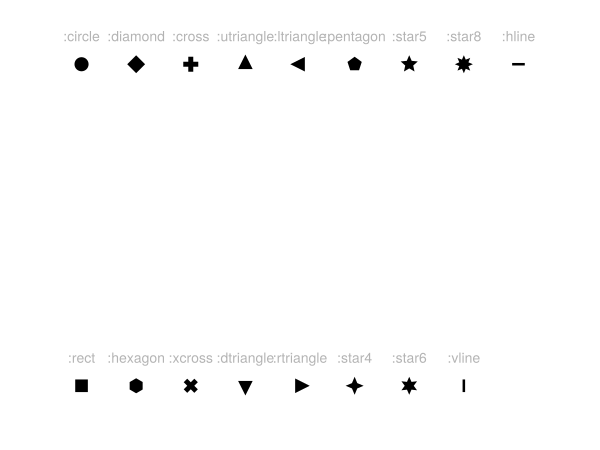
\includegraphics[width=\linewidth]{../figures/markers.pdf}

		\item \jl{markersize} : la taille d'un marqueur.
		\item \jl{strokecolor} et \jl{strokewidth} : couleur et taille (par défaut 0) du pourtour du marqueur.
	\end{itemize}
	\vspace{-1em}

	\begin{minipage}{0.5\linewidth}
		\begin{minted}{julia}
			scatter(x, y;
				markersize=50,
				strokewidth=1,
				marker='Z'
			)
		\end{minted}
	\end{minipage}\hfill%
	\begin{minipage}{0.45\linewidth}
		\includegraphics[width=\linewidth]{../figures/scatter.pdf}
	\end{minipage}
\end{frame}

\begin{frame}[fragile]{Données linéaires simples}
	Spécifiques à \jl{lines} et \jl{scatterlines} :
	\begin{itemize}
		\item \jl{linestyle} : le type de trait, à choisir parmi \jl{:solid} (par défaut), \jl{:dot}, \jl{:dash}, \jl{:dashdot}, \jl{:dashdotdot}, ou bien un tuple avec un des descripteurs précédents et un écart entre les traits, comme \jl{(:dot, 8)}. Voir aussi \jl{Makie.Linestyle} pour plus d'options.
		\item \jl{linewidth} : l'épaisseur de la ligne
	\end{itemize}
	\vfill

	\jl{scatterlines} a aussi un argument \jl{markercolor} qui permet de séparer la couleur des marqueurs de la couleur de la ligne.

	\begin{minipage}{0.5\linewidth}
		\begin{minted}{julia}
			scatterlines(x, y;
				markercolor=:red,
				markersize=20,
				linewidth=6,
				linestyle=(:dashdotdot, 1)
			)
		\end{minted}
	\end{minipage}\hfill%
	\begin{minipage}{0.45\linewidth}
		\includegraphics[width=\linewidth]{../figures/scatterlines.pdf}
	\end{minipage}
\end{frame}

\begin{frame}[fragile]{Histogrammes}
	La fonction \jl{hist} permet d'afficher un histogramme représentant le nombre d'apparitions des éléments d'une liste. Quelques options :
	\begin{itemize}
		\item \jl{weights} : un tableau de nombre de même taille que l'entrée, qui pondère chaque élément par un poids ;
		\item \jl{direction}: \jl{:y} (par défaut) ou \jl{:x} pour des barres horizontales ;
		\item \jl{color}, \jl{strokecolor} et \jl{strokewidth} : comme pour \jl{scatter}
	\end{itemize}

	\begin{minipage}{0.5\linewidth}
		\begin{minted}{julia}
			l = [1, 5, 1, 2, 5]
			weights = [2, 1, 1, 1, 1]

			hist(l;
				weights,
				strokewidth=2,
				direction=:y
			)
		\end{minted}
	\end{minipage}\hfill%
	\begin{minipage}{0.45\linewidth}
		\includegraphics[width=\linewidth]{../figures/hist.pdf}
	\end{minipage}
\end{frame}

\begin{frame}[fragile]{Heatmap}
	La fonction \jl{heatmap} permet d'afficher les valeurs d'une fonction numérique prenant deux arguments, selon une échelle de couleur. Cette échelle est donnée par l'argument \jl{colormap}.

	Les arguments peuvent être donnés de plusieurs façon : le plus simple est de préciser tous les triplets de points $(x, y, z)$ sous la forme de trois vecteurs.

	\begin{minipage}{0.5\linewidth}
		\begin{minted}{julia}
			import Makie.ColorSchemes as CS

			xs = range(0, 2π, length=100)
			ys = range(0, 2π, length=100)
			zs = [sin(x*y) for x in xs,
							   y in ys]

			heatmap(xs, ys, zs;
				colormap=CS.lipari
			)
		\end{minted}
	\end{minipage}\hfill%
	\begin{minipage}{0.45\linewidth}
		\includegraphics[width=\linewidth]{../figures/heatmap.pdf}
	\end{minipage}
\end{frame}

\begin{frame}[fragile]{Dessins superposés}
	Dès que l'on veut ajouter un élément à ces fonctions de base, on doit spécifier explicitement la figure, les axes, et utiliser les fonctions avec un `!' à la fin prenant comme premier argument les axes.

	\begin{minipage}{0.5\linewidth}
		\begin{minted}{julia}
			f = Figure();
			ax = Axis(f[1,1])

			x = [1, 3, 4]; y = [2, -1, 1];
			lines!(ax, x, y)
			lines!(ax, x, [3, 3, 0])

			display(f)
		\end{minted}
	\end{minipage}\hfill%
	\begin{minipage}{0.45\linewidth}
		\includegraphics[width=\linewidth]{../figures/superposed.pdf}
	\end{minipage}

	L'affichage n'a pas lieu avant d'avoir appelé \jl{display(f)}. Dans le REPL, la fonction \jl{display} est automatiquement appelée sur la dernière valeur d'une expression (sauf si cette dernière est suivie d'un `;'), donc il suffit d'entrer \jl{f}. Les fonctions sans `!' renvoient la \jl{Figure}, qui est donc affichée si l'appel de fonction est la dernière expression exécutée du REPL.
\end{frame}

\begin{frame}{Sauvegarder une figure}
	La fonction \jl{save} permet de sauvegarder une figure sous la forme d'un fichier. Plusieurs extensions sont possibles :
	\begin{itemize}
		\item \texttt{.png} : format \emph{matriciel} (tableau de pixels) donc facile à manipuler, sans perte donc lourd.
		\item \texttt{.jpg} : format matriciel compressé, avec perte mais plus léger que .png.
		\item \texttt{.svg} (seulement avec \texttt{CairoMakie}) : format \emph{vectoriel} (courbes paramétriques, notamment de Bézier) donc plus léger pour des figures scientifiques et infiniment précis, manipulable sur un logiciel comme Inkscape.
		\item \texttt{.pdf} (seulement avec \texttt{CairoMakie}) : format vectoriel plus commun, parfois plus léger que \texttt{.svg} mais avec quelques pertes possibles.
	\end{itemize}
	\vfill

	La fonction s'appelle comme \jl{save("/path/to/file.pdf", f)} avec \jl{f} la \jl{Figure}. 
\end{frame}

\begin{frame}[fragile]{Barres d'erreur}
	Superposer des figures permet notamment d'inclure des barres d'erreurs, \textbf{indispensables} sur toute figure scientifique extraite de données obtenues expérimentalement.
	La fonction à utiliser est \jl{errorbars}.

	\begin{minipage}{0.55\linewidth}
		\begin{minted}{julia}
			f = Figure();
			ax = Axis(f[1,1])

			scatter!(ax, x, y; color=:black)
			errorbars!(ax, x, y,
				[0.1, 0.4, 0.2],
				[0.1, 0.1, 0.5]
			)
			errorbars!(ax, x, y, fill(0.1, 3);
				direction=:x,
				color=Makie.wong_colors()[1]
			)

			display(f)
		\end{minted}
	\end{minipage}\hfill%
	\begin{minipage}{0.45\linewidth}
		\includegraphics[width=\linewidth]{../figures/errorbars.pdf}
	\end{minipage}
\end{frame}

\begin{frame}[fragile]{Légende}
	Si une figure représente plusieurs courbes, il faut les légender de façon appropriée. Pour cela, il faut inclure un \jl{label} à chaque fonction d'affichage, et appeler \jl{axislegend} avant d'afficher la figure.	\jl{axislegend} accepte un argument \jl{position}.

	\begin{minipage}{0.55\linewidth}
		\begin{minted}{julia}
			f = Figure();
			ax = Axis(f[1,1])
			
			barplot!(ax, x, y.+2, label="+2")
			barplot!(ax, x, y;
				color=:red,
				label="Raw data"
			)

			# rt : Right Top
			axislegend(ax, position=:rt)
			display(f)
		\end{minted}
	\end{minipage}\hfill%
	\begin{minipage}{0.45\linewidth}
		\includegraphics[width=\linewidth]{../figures/legend.pdf}
	\end{minipage}
\end{frame}

\begin{frame}{Axes}
	La fonction \jl{Axis} accepte des arguments, notamment :
	\begin{itemize}
		\item \jl{xlabel} et \jl{ylabel} : les titres des axes respectivement \texttt{x} et \texttt{y}, sous forme de texte : vos axes \textbf{doivent} être nommés ;
		\item \jl{title} le titre de la figure, sous forme de texte : \textbf{obligatoire} ;
		\item \jl{limits} : un quadruplet \jl{(xmin, xmax, ymin, ymax)}, chacune de ces valeurs pouvant être \jl{nothing} pour laisser le choix automatique ;
		\item \jl{xscale} et \jl{yscale} : au choix entre \jl{identity} (par défaut) et \jl{log10}, et d'autres choix moins courants ;
		\item \jl{xticks} et \jl{yticks} : les valeurs des axes indiquées sur eux, sous la forme d'un vecteur de valeurs, ou d'une paire avec le vecteur des positions et le vecteur des noms affichés.
		\item \jl{xgridvisible} et \jl{ygridvisible} : \jl{true} par défaut.
	\end{itemize}
\end{frame}

\begin{frame}[fragile]{Axes}
	\begin{julia}
		f = Figure();
		ax = Axis(f[1,1];
			title="Evolution of metric deviation with time",
			xlabel="Time (s)", xscale=log10,
			ylabel="Deviation",
			yticks=(0:3, ["Perfect", "Normal", "Poor", "Worst"]),
			limits=(nothing, nothing, 0, 3),
			ygridvisible=false
	\end{julia}
	\begin{minipage}{0.5\linewidth}
		\vspace{-1em}
		\begin{minted}[firstnumber=9]{julia}
			)

			τs = [1, 3, 50, 700_00]
			Δls = [0, 1, 2, 2.5]
			σΔls = [0, 0.1, 0.4, 0.2]

			scatterlines!(ax, τs, Δls)
			errorbars!(ax, τs, Δls, σΔls)

			display(f)
		\end{minted}
	\end{minipage}\hfill%
	\begin{minipage}{0.5\linewidth}
		\includegraphics[width=\linewidth]{../figures/axis.pdf}
	\end{minipage}
\end{frame}

\begin{frame}{Dessin composé}
	Une même figure peut contenir plusieurs axes, chaque axe représentant une sous-figure différente.

	La position des axes est déterminée par le double index utilisé sur la figure : si \jl{f} est une figure, alors \jl{f[1,2]} désigne un espace à droite de \jl{f[1,1]} et de la même hauteur, tandis que \jl{f[0,:]} désigne un espace au-dessus de \jl{f[1,1]}, de la largeur de la figure totale.

	On peut ainsi composer une figure avec un axe principal \jl{Axis(f[1,1])}, une légende à droite \jl{Legend(f[1,2])} et un titre centré \jl{Label(f[0,:])}.
	
	On peut aussi utiliser \jl{Top()}, \jl{Left()}, \jl{BottomRight()}, etc., comme troisième index pour positionner un élément par rapport à un autre.
	\vfill

	Pour préserver l'alignement des axes entre \jl{Axis} voisins, on peut utiliser \jl{linkyaxes!} et \jl{linkxaxes!} au besoin
	\vfill
	
	La taille totale de la figure peut être donnée comme l'argument \jl{size} de \jl{Figure}, par exemple \jl{f = Figure(; size=(600, 450))}.
\end{frame}

\begin{frame}[fragile]{Exemple : figure complexe légendée}
	\begin{minipage}{0.8\linewidth}
		\vspace{0.5em}
		\begin{julia}
			f = Figure(; size=(250, 700));
			ax1 = Axis(f[1, 1], yticklabelcolor = :red)
			ax2 = Axis(f[1, 1], yaxisposition = :right)
			hidespines!(ax2); hidexdecorations!(ax2)
			linkxaxes!(ax1, ax2)
			l1 = lines!(ax1, 0:3, 5:-0.4:3.8, color = :red)
			l2 = scatterlines!(ax2, [1, 5, 7], [0, 1, 4])

			Legend(f[2,1], [l1, l2], ["foo", "bar"])
			Label(f[2,1][0,1], "Légende")
			# make second row smaller than first:
			rowsize!(f.layout, 2, Auto(0.2))

			Label(f[0,1], "The global title")

			Label(f[:,1,TopLeft()], "A";
				font=:bold, fontsize=40)
			
			display(f)
		\end{julia}
	\end{minipage}\hfill%
	\begin{minipage}{0.2\linewidth}
		\includegraphics[height=\textheight]{../figures/composed.pdf}
	\end{minipage}
\end{frame}

\begin{frame}[fragile]{Exemple : heatmap et histogramme}
	\begin{minipage}{\linewidth}
		\vspace{0.5em}
		\begin{julia}
			irange = 0:0.01:2π; jrange = 0:0.01:π
			data = [cos(i*j) for i in irange, j in jrange]

			f = Figure(; size=(700, 200));
			ax1 = Axis(f[1, 1])
			hmap = heatmap!(ax1, irange, jrange, data)

			ax2 = Axis(f[1,0], limits=(-1, 1, 0, π))
			lines!(ax2, cos.(jrange), jrange)
			colsize!(f.layout, 0, Auto(0.5))
			hideydecorations!(ax1); linkyaxes!(ax1, ax2)

			Colorbar(f[1, 2], hmap; label = "Color values")
		\end{julia}
	\end{minipage}

	\begin{minipage}{\linewidth}
		\centering
		\includegraphics[width=0.7\textwidth]{../figures/heatmap2.pdf}
	\end{minipage}
\end{frame}


\begin{frame}[fragile]{Dessin 3D}
	Il est possible de réaliser certains dessins en 3D. Pour cela, il faut remplacer \jl{Axis} par \jl{Axis3} et utiliser des fonctions appropriées comme :
	\begin{itemize}
		\item \jl{wireframe} ou \jl{surface} pour représenter des fonctions de $I\times J$ dans $K$ avec $I$, $J$ et $K$ des sous-ensembles de $\mathbbm R$.
		\item \jl{volume} pour représenter des fonctions de $I\times J\times K$ dans $\mathbbm R$.
		\item \jl{scatter}, \jl{lines} et \jl{scatterlines} sur un \jl{Axis3}.
	\end{itemize}
	\vfill

	Exemple :

	\begin{minipage}{0.65\linewidth}
		\vspace{0.5em}
		\begin{julia}
			f = Figure();
			ax = Axis3(f[1,1], ylabel="prefactor")
			xs = -2:0.1:2; ys = -2:0.3:2;
			zs = [y*sinc(x) for x in xs, y in ys]
			wireframe!(ax, xs, ys, zs, linewidth=1)
			lines!(ax, [-2,2], [0,0], [0,0];
				   color=:red)
			f
		\end{julia}
	\end{minipage}\hfill%
	\begin{minipage}{0.35\linewidth}
		\includegraphics[width=\linewidth]{../figures/wireframe.pdf}
	\end{minipage}
\end{frame}

\begin{frame}[fragile]{Animation}
	Il est possible de créer des animations (c'est-à-dire des courtes vidéos) avec \texttt{Makie.jl}. Pour cela, on appelle la fonction \jl{record} de la forme suivante :
	\JLa{record(update_function, figure, filepath, iterator; framerate)}
	\begin{itemize}
		\item \jl{filepath} est le chemin vers le fichier vidéo à créer.
		\item \jl{figure} est la \jl{Figure} à afficher.
		\item \jl{update_function} est appelée sur chaque valeur de \jl{iterator}, pour modifier \jl{figure}, qui est alors ajoutée à la vidéo.
		\item L'argument optionnel \jl{framerate} contrôle la vitesse de la vidéo.
	\end{itemize}
\end{frame}

\begin{frame}[fragile]{Animation}
	\begin{julia}
		using Makie: ColorSchemes as CS
		f = Figure(); ax = Axis(f[1,1]; limits=(0, 1, 0, 1))
		
		function add_line(x)
			lines!(ax, [0, x], [0,1], color=CS.lipari[x])
		end
		
		record(add_line, f, "/tmp/animation.mkv", 0:0.01:1)
	\end{julia}

	\begin{minipage}{\linewidth}
		\centering
		\includegraphics[width=0.5\linewidth]{../figures/animation_lines.pdf}
	\end{minipage}
\end{frame}

\begin{frame}[fragile]{Animation}
	Pour faire des animations plus compliquées, on utilise \jl{Observable} pour définir une valeur spéciale qui sera mise à jour par la fonction donnée en premier argument à \jl{record}.

	Pour utiliser cette valeur, chaque argument d'une fonction de \texttt{Makie.jl} la contenant doit être préfixée par la macro \jl{@lift}. Le nom de l'\jl{Observable} doit être préfixé par un \mintinline{julia}|$|, comme une interpolation de chaîne de caractères.

	\begin{julia}
		using Makie: ColorSchemes as CS
		f = Figure(); ax = Axis(f[1,1]; limits=(0, 1, 0, 1))

		time = Observable(0.0)

		xs = @lift [0, $time]
		ys = [0, 1]
		color = @lift CS.lipari[$time]
		lines!(ax, xs, ys; color)
		
		record(t -> (time[] = t), f, "/tmp/animation2.mkv", 0:0.01:1)
	\end{julia}
\end{frame}

\end{document}